
\chapter{INTRODUCTION}

Co-channel speech refers to single-channel audio signals that contain more than one speaker. 
A wide range of terms have been used to describe various aspects of co-channel speech, 
which will be clarified throughout this chapter. 
We consider both conversational speech and artificially mixed streams as co-channel. 
All signals treated in this study are single-channel recordings. 
Of all such data, a subset may have more than one ``active'' speaker at the same time, i.e. multi-speaker segments, 
which we label as ``overlapped speech''. 
Overlapped regions are segments of a co-channel signal where both speakers are simultaneously active. This categorization is summarized in Fig.~\ref{fig:cochannel_vs_overlap}.

% FIX CROPPING ON MAC
\begin{figure}[h!]
	\centering
	\vspace{0mm}
	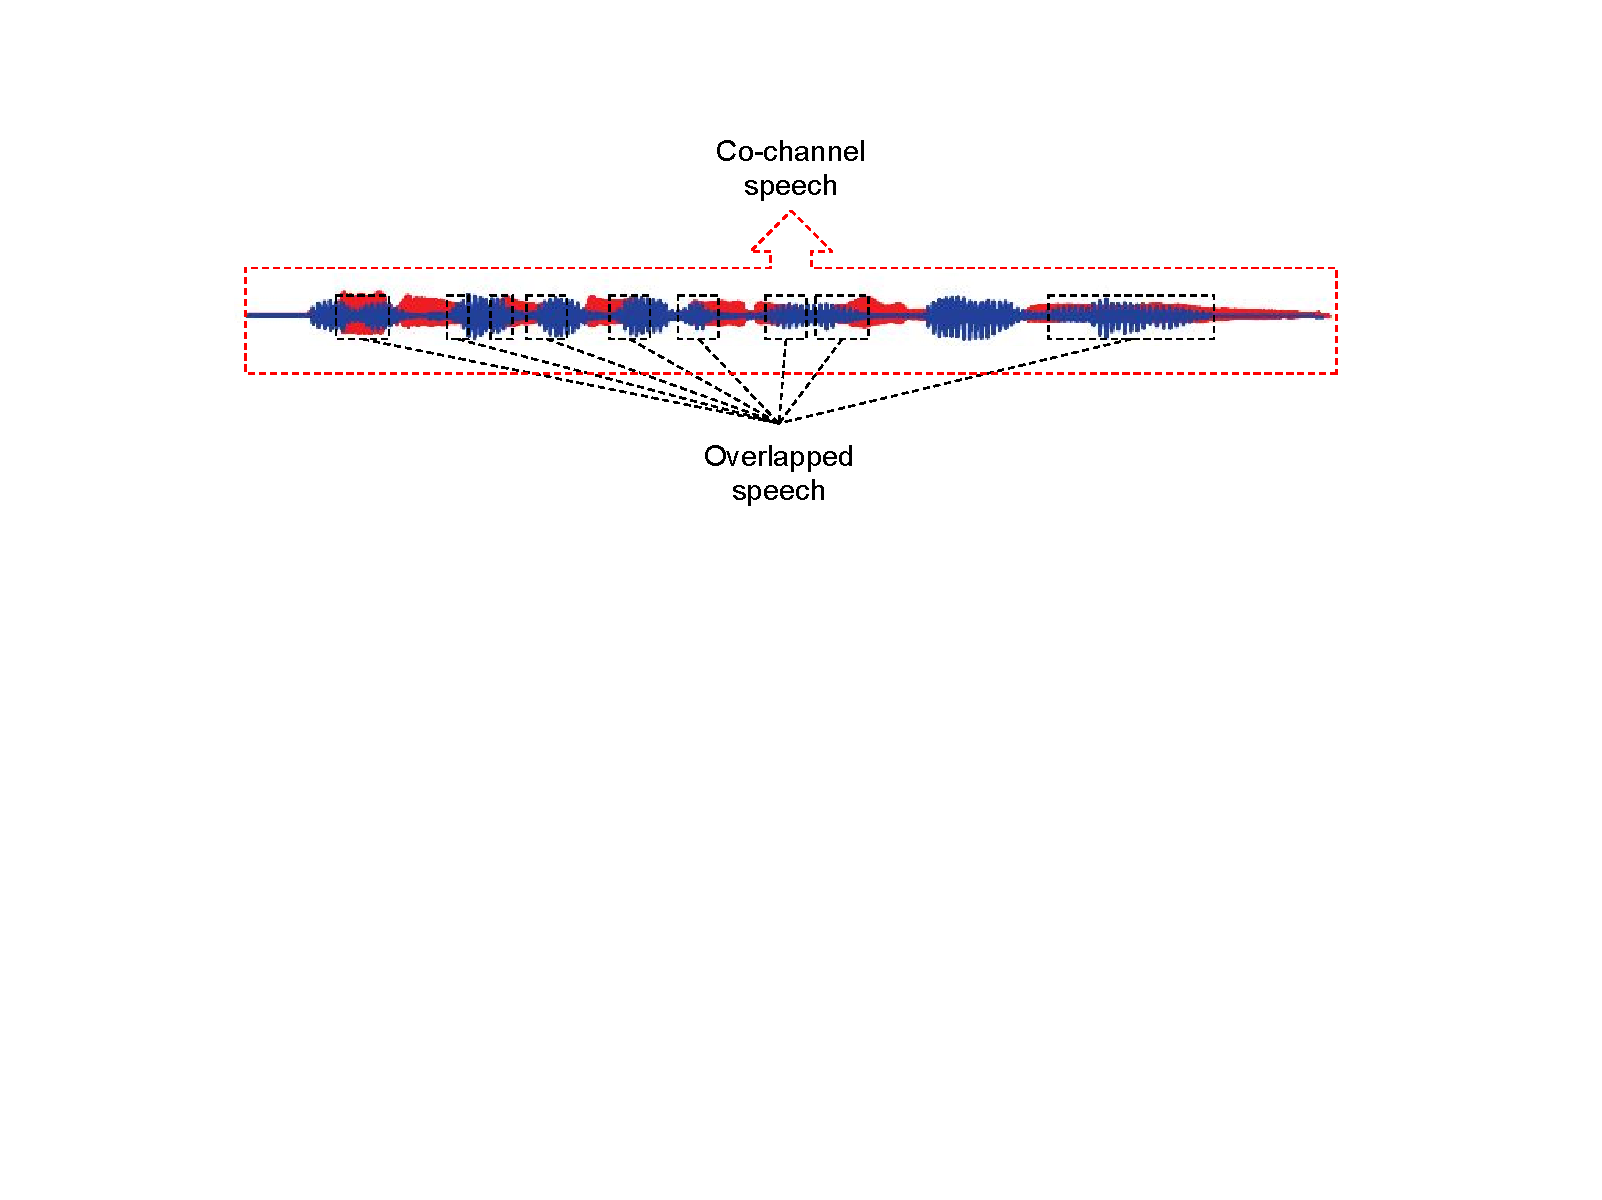
\includegraphics[height = 3in, width=0.9\textwidth]{figures/cochannel_vs_overlap-crop}
	\vspace{-3mm}
	\caption{Difference between co-channel and overlapped speech. Overlap refers to instances where more than one speaker is active. Co-channel is defined as an entire stream that contains multiple speakers. All co-channel files do not necessarily contain overlap. }
	\label{fig:cochannel_vs_overlap}
	\vspace{-3mm}
\end{figure}


%The specifics of recording conditions are overlooked in this study. 
%For example, information that relates to each speaker’s distance from the microphone and room acoustics. 
%This is intentional, since most of the difficulty in dealing with co-channel speech arises 
%from it being single-channel, which implies limited access to spatial 
%information as well as other sources of meta-data.

There are different ways of categorizing co-channel data in terms of how it is generated. This study considers a semantic classification that focuses on speakers' interactions with each other. We divide co-channel data into two subgroups: 
\begin{itemize}
	\item conversational co-channel speech
	\item co-channel speech with independent parties
\end{itemize} 

Conversational co-channel speech refers to recordings in which speakers acknowledge other parties in the recording and engage in dialog. 
Alterations of speech production are an important artifact of conversational co-channel speech, which are the result of conscious and unconscious reactions of the foreground speaker and interferer(s) during speech especially at or around overlaps. 
Examples of such alterations are raised pitch and energy level [2]. 
Political debates are filled with arguments between rival candidates. 
Debates can be perfect examples of an exaggerated version of the above-mentioned changes in speech production. 
Speakers tend to alter their voice in order to control the floor in such ``conversations''. 
These changes are problematic in automatic speech applications and are considered a type of distortion. 
Consequently, the treatment will be directed towards applications that suffer the most from such alterations, predominantly speech recognition. 
Obviously, aside from changes in each speaker's voice, the element of interference by competing speakers also introduces overlaps. 
Therefore, in conversational co-channel data, one has to consider both overlaps and speaker specific alterations as sources of distortion and mismatch. 

Co-channel data with independent parties, are examples of co-channel data where the speakers do not interact with each other. 
Cross-talk between separate channels is considered a source of such co-channel speech. 
The main characteristic of such data is that speakers are not aware of each other and therefore do not pertain to normal conversational mannerisms. 
That includes following turn-taking rules, which in most cases limits overlapped speech. 
Artificially generated co-channel data (mixing independent channels) is another example of co-channel speech with independent parties. 
A considerable portion of this study will focus on this type of artificially generated co-channel data to analyze performance of overlap detection and also speaker recognition. 
We rely on this data since it provides the flexibility of controlling the amount of overlapped speech. 
As we will show in this chapter, conversational co-channel speech does not necessarily contain sufficient overlapped data for some of our experiments. 
The main source of distortion in independent party co-channel speech is considered overlapped speech. 
This allows an isolated treatment of overlap, which is considered a main focus in this study. 

\section{Background}
\label{sec:background}



\section{Approach}

The goal of this thesis is to provide tangible solutions to problems caused by co-channel speech in automatic speech technology. 
We argue that part of these issues are caused by overlapped speech (direct speech interference) and the remaining are a result of multiple speakers in audio streams. 
Both of which reduce the reliability of trained acoustic models while at the same time adding interference to test data. 
We will address different ways of removing such interferences; in the signal level and also in model subspaces. 

The presence of overlapped speech can be detrimental to speaker diarization and speech recognition systems. 
There is no clear and unique way of labeling or transcribing overlapped segments. 
In speaker diarization, it becomes difficult to assess system performance at overlaps. 
The same goes for speech recognition. 
Since aside from determining which is the ``primary'' speaker, recognizing speech at overlaps is more difficult due to interference from ``interfering'' speakers. 
For this and other reasons detailed in the next chapter, the first portion of this study is devoted to overlapped speech detection. 
Our approach to overlap detection will be to focus on developing signal processing techniques to detect and separate overlapped from single speaker speech. 

Aside from overlaps, in many applications, such as speaker recognition, the mere presence of interfering speakers is a nuisance. 
In fact, in many conversational speaker recognition corpora, the amount of overlap in co-channel data is negligible. 
Therefore, we propose using techniques to remove interfering speakers from co-channel data. 
This is performed in two different ways: 
\begin{itemize}
\item Remove interfering speakers in the signal level: speaker diarization.
\item Remove interfering speakers in the feature subspace: i-vector subspace factorization.
\end{itemize}

Each of these methods will be described in a separate chapter. 
Speaker diarization, will attempt to recognize and group speech that belongs to the same speaker in a co-channel audio stream. 
While subspace factorization maps speaker dependent models to a subspace that will only contain parameters identifying the speaker of interest (aka primary speaker). 


 
